% !TeX spellcheck = en_US
\section{Problem 2}
Second-order optimization methods are a class of algorithms used for finding the minimum or maximum of a function. These methods are characterized by their use of second-order derivatives, specifically the $Hessian \ \ matrix$, which contains the second partial derivatives of the function being optimized. The use of that method takes into account the curvature of the function.\\

One of the most well-known second-order methods is Newton's method. It updates the paarameters by moving in the direction of the inverse Hessian matrix applied to the gradient.\\

The update rule is given by:
\begin{equation}
	x_{k+1} = x_k - H^{-1}\nabla F(x_k)
\end{equation}
where
\begin{itemize}
	\item $x_k$ is the parameter vector at iteration $k$
	\item $\nabla F(x_k)$ is the gradient and
	\item $ H^{-1}$ is the inverse of the Hessian matrix at $x_k$
\end{itemize}
\vspace{2mm}
With that being said, we need to find the minimum of the function
\begin{equation}	
	F(\mathbf{w})=w_{1}^{2}+w_{2}^{2}+(0.5w_{1}+w_{2})^{2}+(0.5w_{1}+w_{2})^{4}	
	\label{eq:Equation2}
\end{equation}


using the Newton method and fixed step $\lambda = 1$, even though this is not a quadratic form.\\

To implement the code we followed the algorithm's basic steps:\\

\underline{Step 1}: Calculate gradient $\mathbf{\nabla F(x_k)}$ and Hessian matrix $\mathbf{\nabla^2F(x_k)}$ \\

\underline{Step 2}: If we have no-quadratic form, find and calculate Inversive Hessian Matrix $\mathbf{H^{-1}}$\\

\underline{Step 3}: Compute the minimizing direction $\mathbf{s_{k}}$\\
The formula for the minimizing direction $s_{k}$ is
\begin{equation}
	\begin{gathered}
		s_{k} = \left[-\nabla^2F(x_k)\right]^{-1} \cdot \nabla F(x_k)\\
		\text{or for simplicity}\\
		s_{k} = -H^{-1} \cdot \nabla F(x_k)
	\end{gathered}
\end{equation}

\underline{Step 4}: Minimize $\mathbf{F(x_{k} + \lambda_{k} \cdot s_{k})}$ to find optimal $\lambda_{k}$\\
There are two ways to do it
\begin{itemize}
	\item By $\dfrac{d f(x_k - \lambda_k [\nabla^2 f(x_k)]^{-1} \nabla f(x_k))}{d \lambda_k} = 0$ or
	\item By using a 1D optimization method
\end{itemize}
Keep in mind that if our equation is in quadratic form we always suppose that $\lambda = 1$.\\
On our exercise, even though Equation~\ref{eq:Equation2} is not on quadratic form, we suppose that $\lambda$ has a fixed value of 1.\\

\underline{Step 5:} Calculate the next point $\mathbf{x_{k+1}}$\\
Each time, to find the next point we calculate:
\begin{equation}
	x_{k+1} = x_{k} + \lambda_{k} \cdot s_{k}
\end{equation}

\underline{Step 6:} Check convergence criterion\\
A condition that determines when an iterative process should stop because it has reached a solution that is close enough to the exact solution. \\
Hence, we define the tolerance: $\epsilon = 10^{-6}$
\vspace{2mm}

Everything considered, we implement these steps into \textit{"Newton.m"} and we conclude into the fact that:\\
\begin{enumerate}
	\item The minimum of the function occurs at $1.0e-12*$ with $\mathbf{x_{k} = [0.1055; 0.2109]}$\\
	This is the point where the minimum of the function occurs. The numbers $0.1055$ and $0.2109$ are the $x1$ and $x2$ coordinates of the minimum point, respectively. The $1.0e-12*$ indicates that these numbers are in the order of $10^{-12}$, so the actual coordinates are extremely close to zero, as we want to.
	\item The number of iterations is: $\mathbf{8}$
\end{enumerate}

We can visualize these results with the help of the following plots.

\begin{figure}[H]
	\centering
	\begin{subfigure}{0.45\textwidth}
		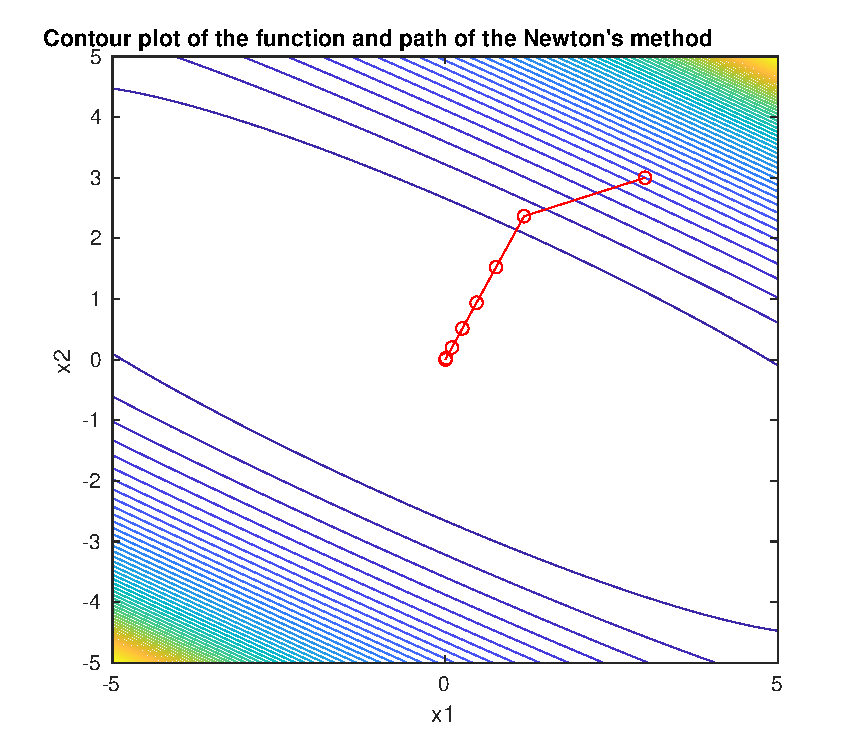
\includegraphics[width=\textwidth]{../Problem 2/contour_plot.pdf}
		\caption{Contour plot of the $F(w)$ function with path trajectory}
	\end{subfigure}
	\quad
	\begin{subfigure}{0.5\textwidth}
		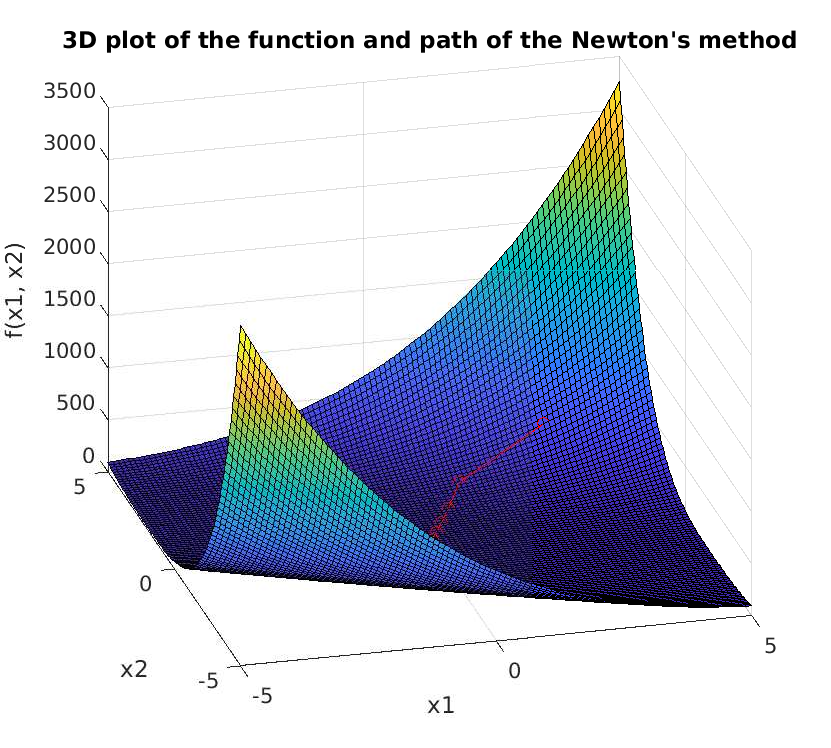
\includegraphics[width=\textwidth]{../Problem 2/3D_plot.pdf}
		\caption{3D visualization}
	\end{subfigure}
\end{figure}
\vspace{3mm}
The path represents the sequence of points visited by Newton's method as it converges to the minimum $[0; 0]$, highlighting the method's efficiency and directionality in navigating the function's terrain towards the optimum.\\

By comparing the Newton method with the previous ones, the Conjugate Gradient and the Gradient Descent method for solving optimization problems, several key differences and insights emerge:
\begin{enumerate}
	\item Convergence speed:\\
	The Newton method offers quadratic convergence under suitable conditions, which means it can converge to the solution in fewer iterations compared to CG and GD, especially when close to the optimum. However, this rapid convergence comes at the cost of calculating and inverting the Hessian matrix, which can be computationally expensive for high-dimensional problems.
	\item Computational complexity:\\
	Newton has high computational cost due to the necessity of computing and inverting the Hessian matrix at each iteration, in contrast with Conjugate gradient that does not require explicit computations for it. The Gradient Descent has the lowest computational cost per iteration among the three, as it only requires the calculation of the gradient. However, it may require more iterations to converge.
	\item Memory usage:\\
	The method that has the most requirements is the Newton method, because it requires more memory to store the Hessian matrix and its reverse. Next comes Conjugate gradient and at last Gradient Descent method has in general low memory requirements.
\end{enumerate}

In summary, we can conclude that the Gradient Descent method is the simplest algorithm among these three, the Conjugate gradient is more suitable for large-scale problems and the Newtons method is the fastest one. We understood that, because for the same function the one that converged first was the Newton's application. 



